\begin{figure}[t]
  \begin{center}
    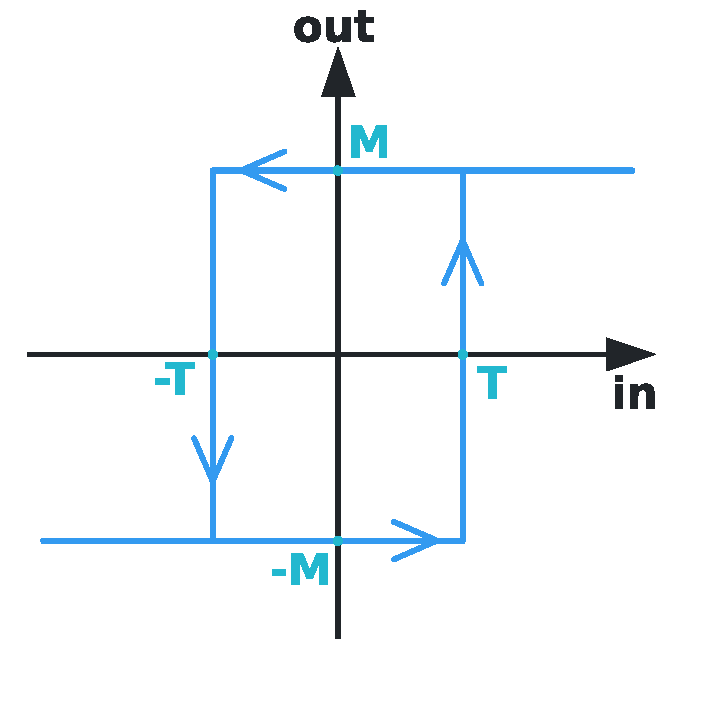
\includegraphics[width=0.382\textwidth]{VBA/1/Hysteresis}
  \end{center}
  \caption{Vereinfachte Kennlinie eines (nichtinvertierenden) Schmitt-Triggers (Quelle: Wikipedia)}
\end{figure}
Ein Schmitt-Trigger ist eine Art des Komparators, dessen Ein-Ausgangs-Kennlinie
einer Hysterese unterliegt, welche durch zwei Schwellenwerte charakterisiert ist.


Gerät die (analoge) Eingangsspannung über den oberen Schwellwert \textit{T} läuft die
Ausgangsspannung des Triggers auf ihren maximalen positiven Wert \textit{M} (Sättigung). In diesem
Fall bewirkt die weitere Erhöhung der Eingangsspannung keine Veränderung der
Ausgangsspannung. Erst wenn der Eingangsspannungswert auf den unteren
Schwellwert \textit{$-T$} abfällt, ändert sich die Ausgangsspannung auf den
maximal negativen Wert \textit{$-M$}. Analog gilt hier, dass sich erst bei
Überschreitung der oberen Schwelle die Ausgangsspannung wieder ändert. 

Ein Schmitt-Trigger kann beispielsweise mithilfe eines positiv-rückgekoppelten
Operationsverstärkers realisiert werden.
